%%%%%%%%%%%%%%%%%%%%%%%%%%%%%%%%%%%%%%%%%
% Short Sectioned Assignment
% LaTeX Template
% Version 1.0 (5/5/12)
%
% This template has been downloaded from:
% http://www.LaTeXTemplates.com
%
% Original author:
% Frits Wenneker (http://www.howtotex.com)
%
% License:
% CC BY-NC-SA 3.0 (http://creativecommons.org/licenses/by-nc-sa/3.0/)
%
%%%%%%%%%%%%%%%%%%%%%%%%%%%%%%%%%%%%%%%%%

%----------------------------------------------------------------------------------------
%	PACKAGES AND OTHER DOCUMENT CONFIGURATIONS
%----------------------------------------------------------------------------------------

\documentclass[paper=a4, fontsize=11pt]{scrartcl} % A4 paper and 11pt font size

\usepackage[T1]{fontenc} % Use 8-bit encoding that has 256 glyphs
\usepackage[ngerman]{babel}
\usepackage{fourier} % Use the Adobe Utopia font for the document - comment this line to return to the LaTeX default
\usepackage{amsmath,amsfonts,amsthm} % Math packages
\usepackage{graphicx}
\usepackage[utf8]{inputenc}
\usepackage{listings}
\usepackage[section]{placeins}
\usepackage{lipsum} % Used for inserting dummy 'Lorem ipsum' text into the template
\usepackage{float}
\usepackage{multicol}
\usepackage{algpseudocode}
\usepackage{algorithm}% http://ctan.org/pkg/algorithms

% Algorithmic modifications
\makeatletter
\newcommand{\ALOOP}[1]{\ALC@it\algorithmicloop\ #1%
  \begin{ALC@loop}}
\newcommand{\ENDALOOP}{\end{ALC@loop}\ALC@it\algorithmicendloop}
\renewcommand{\algorithmicrequire}{\textbf{Input:}}
\renewcommand{\algorithmicensure}{\textbf{Output:}}
\newcommand{\algorithmicbreak}{\textbf{break}}
\newcommand{\BREAK}{\STATE \algorithmicbreak}
\makeatother

\usepackage{sectsty} % Allows customizing section commands
\allsectionsfont{\centering \normalfont\scshape} % Make all sections centered, the default font and small caps

\usepackage{fancyhdr} % Custom headers and footers
\pagestyle{fancyplain} % Makes all pages in the document conform to the custom headers and footers
\fancyhead{} % No page header - if you want one, create it in the same way as the footers below
\fancyfoot[L]{} % Empty left footer
\fancyfoot[C]{} % Empty center footer
\fancyfoot[R]{\thepage} % Page numbering for right footer
\renewcommand{\headrulewidth}{0pt} % Remove header underlines
\renewcommand{\footrulewidth}{0pt} % Remove footer underlines
\setlength{\headheight}{13.6pt} % Customize the height of the header

\numberwithin{equation}{section} % Number equations within sections (i.e. 1.1, 1.2, 2.1, 2.2 instead of 1, 2, 3, 4)
\numberwithin{figure}{section} % Number figures within sections (i.e. 1.1, 1.2, 2.1, 2.2 instead of 1, 2, 3, 4)
\numberwithin{table}{section} % Number tables within sections (i.e. 1.1, 1.2, 2.1, 2.2 instead of 1, 2, 3, 4)

\setlength\parindent{0pt} % Removes all indentation from paragraphs - comment this line for an assignment with lots of text

\DeclareMathOperator*{\argmin}{arg\,min}

%----------------------------------------------------------------------------------------
%	TITLE SECTION
%----------------------------------------------------------------------------------------

\newcommand{\horrule}[1]{\rule{\linewidth}{#1}} % Create horizontal rule command with 1 argument of height

\title{
\normalfont \normalsize
\textsc{Karlsruhe Institute of Technology} \\ [25pt] % Your university, school and/or department name(s)
\horrule{0.5pt} \\[0.4cm] % Thin top horizontal rule
\huge Nichtlineare Optimierung\\ Zusammenfassung WS17/18 % The assignment title
\horrule{2pt} \\[0.5cm] % Thick bottom horizontal rule
}

\author{Manuel Lang} % Your name

\date{\normalsize\today} % Today's date or a custom date

\begin{document}

\maketitle % Print the title
%\newpage
%\tableofcontents
%\newpage

\section{Einführung}

\subsection{Begriffe}

\begin{itemize}
\item $\bar{x}$ heißt \textit{lokaler Minimalpunkt} von $f$ auf $M$, falls eine Umgebung $U$ von $\bar{x}$ mit $\forall x \in U \cap M: f(x) \ge f(\bar{x})$ existiert.
\item $\bar{x}$ heißt \textit{globaler Minimalpunkt} von $f$ auf $M$, falls man obig $U = \mathbb{R}^n$ wählen kann.
\item Ein lokaler oder globaler Minimalpunkt heißt \textit{strikt}, falls obig für $x \neq \bar{x}$ sogar die strikte Ungleichung $>$ gilt.
\item Zu jedem globalen Minimalpunkt $\bar{x}$ heißt $f(\bar{x}) (=v= \min\limits_{x \in M} f(x))$ \textit{globaler Minimalwert}, und zu jedem lokalen Minimalpunkt $\bar{x}$ heißt $f(\bar{x})$ \textit{lokaler Minimalwert}.
\item Funktion nicht differenzierbar $\implies$ nichtglattes Optimierungsproblem
\item Euklidsche Norm lässt sich durch Quadrieren (Weglassen der Wurzel) zu glattem Problem umformen (optimale Punkte bleiben erhalten)
\end{itemize}

\subsection{Lösbarkeit}

\begin{itemize}
\item $\alpha \in \mathbb{R}$ wird als \textit{untere Schranke} für $f$ auf $M$ bezeichnet, falls $\forall x \in M: \alpha \le f(x)$ gilt.
\item Das Infimum von $f$ auf $M$ ist die \textit{größte} untere Schranke von $f$ auf $M$, es gilt also $v = inf_{x \in M} f(x)$ falls $v \le f(x)$ für alle $x \in M$ gilt (d.h. $v$ ist selbst untere Schranke von $f$ auf $M$) und $\alpha \le$ für alle unteren Schranken $\alpha$ von $f$ auf $M$ gilt.
\item Definition Lösbarkeit: Das Minimierungsproblem $P$ heißt \textit{lösbar}, falls es ein $\bar{x}$ mit $inf_{x \in M} f(x) = f(\bar{x})$ existiert.
\item Satz: \textit{Das Minimierungsproblem $P$ ist genau dann lösbar, wenn es einen globalen Minimalpunkt besitzt.}
\item Satz von von Weierstraß: \textit{Die Menge $M \subseteq \mathbb{R}^n$ sei nichtleer und kompakt, und die Funktion $f: M \rightarrow \mathbb{R}$ sei stetig. Dann besitzt $f$ auf $M$ (mindestens) einen globalen Minimalpunkt und einen globalen Maximalpunkt.}
\item Definition untere Niveamenge: Für $ \subseteq \mathbb{R}^n, f:X \rightarrow \mathbb{R}$ und $\alpha \in \mathbb{R}$ heißt $lev^\alpha_\le(f,X) = \{ x \in X | f(x) \le \alpha \} $ \textit{untere Niveaumenge von $f$ auf $X$ zum Niveau $\alpha$}. Im Fall $X = \mathbb{R}^n$ schreiben wir auch kurz $f^\alpha_\le := lev^\alpha_\le (f,\mathbb{R}^n) ( = \{ x \in \mathbb{R}^n | f(x) \le \alpha \} )$.
\item Wir führen die Menge der globalen Punkte $S = \{ \bar{x} \in M | \forall x \in M: f(x) \ge f(\bar{x}) \}$ von $P$ ein.
\item Lemma: \textit{Für ein $\alpha \in \mathbb{R}$ sei $lev^\alpha_\le (f,M) \neq \emptyset$. Dann gilt $S \subseteq lev^\alpha_\le (f,M)$.}
\item Verschärfter Satz von Weierstraß: \textit{Für eine (nicht notwendiger beschränkte oder abgeschlossene) Menge $M \subseteq \mathbb{R}^n$ sei $f: M \rightarrow \mathbb{R}$ stetig, und mit einem $\alpha \in \mathbb{R}$ set $lev^\alpha_\le(f,M)$ nichtleer und kompakt. Dann besitzt $f$ auf $M$ (mindestens) einen globalen Minimalpunkt.}
\item Korollar (Verschärfter Satz von Weierstraß für unrestringierte Probleme): \textit{Die Funktion $f: \mathbb{R}^n \rightarrow \mathbb{R}$ sei stetig, und mit einem $\alpha \in \mathbb{R}$ sei $lev^\alpha_\le$ nichtleer und kompakt. Dann besitzt $f$ auf $\mathbb{R}^n$ (mindestens) einen globalen Minimalpunkt.}
\item Definition Koerzivität: Gegeben sei eine abgeschlossene Menge $X \subseteq \mathbb{R}^n$ und eine Funktion $f:X \rightarrow \mathbb{R}$. Falls für alle Folgen $(x^k) \subseteq X$ mit $lim_k ||x^k|| = +\infty$ auch $lim_k f(x^k) = + \infty$ gilt, dann heißt f \textit{koerziv} auf X.
\item Lemma: \textit{Die Funktion $f: X \rightarrow \mathbb{R}$ sei stetig und koerziv auf der (nicht notwendigerweise beschränkten) abgeschlossenen Menge $X \subseteq \mathbb{R}^n$. Dann ist die Menge $lev^\alpha_\le(f,X)$ für jedes Niveau $\alpha \in \mathbb{R}$ kompakt}.
\item Korollar: \textit{Es sei $M$ nichtleer und abgeschlossen, aber nicht allsectionsfont beschränkt. Fernser sei die Funktion $f: M \rightarrow \mathbb{R}$ stetig und koerziv auf $M$. Dann besitzt $f$ auf $M$ (mindestens) einen globalen Minimalpunkt.}
\end{itemize}

\subsection{Rechenregeln und Umformungen}

\begin{itemize}
\item Skalare Vielfache und Summen
\begin{itemize}
\item $\forall \alpha \ge 0, \beta \in \mathbb{R}$: $min_{x \in M} (\alpha f(x) + \beta) = \alpha (min_{x \in M} f(x)) + \beta$.
\item $\forall \alpha \le 0, \beta \in \mathbb{R}$: $min_{x \in M} (\alpha f(x) + \beta) = \alpha (max_{x \in M} f(x)) + \beta$.
\item $min_{x \in M} (f(x) + g(x)) \ge min_{x \in M} f(x) + min_{x \in M} g(x)$.
\item In obiger Ungleichung kann der strikte Fall $>$ auftreten.
\item In den ersten beiden Zeilen stimmen die lokalen bzw. globalen Optimalpunkte der Optimierungsprobleme überein.
\end{itemize}
\item Separable Zielfunktion auf kartesischem Punkt
\begin{itemize}
\item Es seien $X \subseteq \mathbb{R}^n, Y \subseteq \mathbb{R}^m, f: X \rightarrow \mathbb{R}$ und $g: Y \rightarrow \mathbb{R}$. Dann gilt $\min\limits_{(x,y)\in X x Y} (f(x) + g(y)) = \min\limits_{x \in X} f(x) + \min\limits_{y \in Y} g(y)$
\end{itemize}
\item Vertauschung von Minima und Maxima
\begin{itemize}
\item Es seien $X \subseteq \mathbb{R}^n, Y \subseteq \mathbb{R}^m, M = X x Y$ und $f: M \rightarrow \mathbb{R}$ gegeben. Dann gilt:
\item $min_{(x,y)\in M}f(x,y) = min_{x \ in X} min_{y \in Y} f(x,y) = min_{y \in Y} min_{x \in X} f(x,y)$.
\item $max_{(x,y)\in M}f(x,y) = max_{x \ in X} max_{y \in Y} f(x,y) = max_{y \in Y} max_{x \in X} f(x,y)$.
\item $min_{x \in X} max_{y \in Y} f(x,y) \ge max_{y \in Y} min_{x \in X} f(x,y)$.
\item In obiger Ungleichung kann der strikte Fall $>$ auftreten.
\end{itemize}
\item Monotone Transformation: Zu $M \subseteq \mathbb{R}^n$ und einer Funktion $f: M \rightarrow Y$ mit $Y \subseteq \mathbb{R}$ sei $\psi : Y \rightarrow \mathbb{R}$ eine streng monoton wachsende Funktion. Dann gilt $\min\limits_{x \in M} \psi(f(x)) = \psi(\min\limits_{x \in M} f(x))$, und die lokalen bzw. globalen Minimalpunkte stimmen überein.
\item Epigrahumformulierung: Gegeben seien $M \subseteq \mathbb{R}^n$ und eine Funktion $f: M \mathbb{R}$. Dann sind die Probleme $P: \min\limits_{x \in \mathbb{R}^n} f(x)$ s.t. $x \in M$ und $P_{epi}: \min\limits_{x,\alpha \in \mathbb{R}^n x \mathbb{R}} \alpha$ s.t. $f(x) \le \alpha, x \in M$ in folgendem Sinne äquivalent.
\begin{itemize}
\item Für jeden lokalen bzw. globalen Minimalpunkt $x^*$ von $P$ ist $(x^*,f(x^*))$ lokaler bzw. globaler Minimalpunkt von $P_{epi}$.
\item Für jeden lokalen bzw. globalen Minimalpunkt $(x^*,\alpha^*)$ von $P_{epi}$ ist $x^*$ lokaler bzw. globaler Minimalpunkt von $P$.
\item Die Minimalwerte von $P$ und $P_{epi}$ stimmen überein.
\end{itemize}
\item Definition Parallelprojektion: Es sei $M \subseteq \mathbb{R}^n x \mathbb{R}^m$. Dann heißt $pr_x M = \{ x \in \mathbb{R}^n | \exists y \in \mathbb{R}^m : (x,y) \in M \}$ Parallelprojektion von $M$ auf den \glqq x-Raum \grqq $\mathbb{R}^n$.
\item Projektionsumformulierung: Gegeben seien $M \subseteq \mathbb{R}^n x \mathbb{R}^m$ und eine Funktion $f: \mathbb{R}^n \rightarrow \mathbb{R}$, die nicht von den Variablen aus $\mathbb{R}^m$ abhängt. Dann sind die Probleme $P: \min\limits_{(x,y) \in \mathbb{R}^n x \mathbb{R}^m} f(x)$ s.t. $(x,y) \in M$ und $P_{proj}: \min\limits_{x \in \mathbb{R}^n} f(x)$ s.t. $x \in pr_x M$ in folgendem Sinne äquivalent:
\begin{itemize}
\item Für jeden lokalen bzw. globalen Minimalpunkt $(x^*,y^*)$ von $P$ ist $x^*$ lokaler bzw. globaler Minimalpunkt von $P_{proj}$.
\item Für jeden lokalen bzw. globalen Minimalpunkt $x^*$ von $P_{proj}$ existiert ein $y^* \in \mathbb{R}^n$, sodass $(x^*,y^*)$ lokaler bzw. globaler Minimalpunkt von $P$ ist.
\item Die Minimalwerte von $P$ und $P_{proj}$ stimmen überein.
\end{itemize}
\end{itemize}

\section{Unrestringierte Optimierung}

\subsection{Optimalitätsbedingungen}

\subsubsection{Abstiegsrichtungen}

\begin{itemize}
\item Definition Abstiegsrichtung: Es seien $f: \mathbb{R}^n \rightarrow \mathbb{R}$ und $\bar{x} \in \mathbb{R}^n$. Ein Vektor $d \in \mathbb{R}^n$ heißt \textit{Abstiegsrichtung} für $f$ in $\bar{x}$ falls $\exists \check{t} > 0 \forall t \in (0, \check{t}): f(\bar{x} + td) < f(\bar{x})$ gilt.
\item Definition eindimensionale Einschränkung: Gegeben seien $f: \mathbb{R}^n \rightarrow \mathbb{R}$, ein Punkt $\bar{x} \in \mathbb{R}^n$ und ein Richtungsvektor $d \in \mathbb{R}^n$. Die Funktion $\phi_d : \mathbb{R}^1 \rightarrow \mathbb{R}^1, t 	\mapsto f(\bar{x} + td)$ heißt \textit{eindimensionale Einschränkung} von $f$ auf die durch $\bar{x}$ in Richtung $d$ verlaufende Gerade.\\
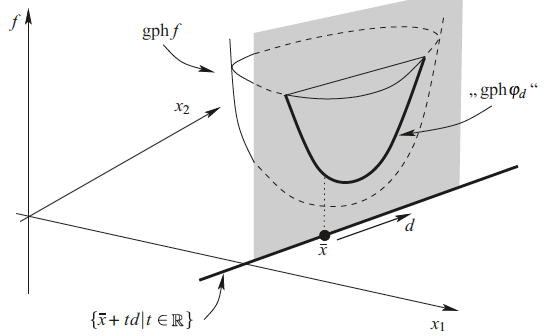
\includegraphics[width=0.5\textwidth]{imgs/eindimeinschr}
\end{itemize}

\subsubsection{Optimimalitätsbedingung erster Ordnung}

\begin{itemize}
\item Definition einseitige Richtungsbleitung: Eine Funktion $f : \mathbb{R}^n \rightarrow \mathbb{R}$ heißt an $\bar{x} \in \mathbb{R}^n$ in eine Richtung $d \in \mathbb{R}^n$ \textit{einseitig richtungsdifferenzierbar}, wenn der Grenzwert $f'(\bar{x},d) := \lim\limits_{t \searrow 0} \frac{f(\bar{x} + td) - f(\bar{x})}{t}$ existiert. Der Wert $f'(\bar{x},d)$ heißt dann \textit{einseitige Richtungsableitung}. Die Funktion $f$ heißt an $\bar{x}$ \textit{einseitig richtungsdifferenzierbar}, wenn $f$ an $\bar{x}$ in jede Richtung $d \in \mathbb{R}^n$ einseitung richtungsdifferenzierbar ist, und $f$ heißt \textit{einseitig richtungsdifferenzierbar}, wenn $f$ an jedem $\bar{x} \in \mathbb{R}^n$ einseitig richtungsdifferenzierbar ist.
\item Lemma: Die Funktion $f: \mathbb{R}^n \rightarrow R$ sei an $\bar{x} \in \mathbb{R}^n$ in Richtung $d \in \mathbb{R}^n$ einseitig richtungsdifferenzierbar mit $f'(\bar{x},d) < 0$. Dann ist $d$ Abstiegsrichtung für $f$ in $\bar{x}$.
\item Lemma: Die Funktion $f: \mathbb{R}^n \rightarrow \mathbb{R}$ sei an einem lokalen Minimalpunkt $\bar{x} \in \mathbb{R}^n$ einseitig richtungsdifferenzierbar. Dann gilt $f'(\bar{x},d) \ge 0$ für jede Richtung $d \in \mathbb{R}^n$.
\item Definition Abstiegsrichtung erster Ordnung: Für eine am Punkt $\bar{x} \in \mathbb{R}^n$ in Richtung $d \in \mathbb{R}^n$ einseitig richtungsdifferenzierbare Funktion $f: \mathbb{R}^n \rightarrow \mathbb{R}$ heißt $d$ \textit{Abstiegsrichtung erster Ordnung}, falls $f'(\bar{x},d) < 0$ gilt.
\item Definition stationärer Punkt: Die Funktion $f: \mathbb{R}^n \rightarrow \mathbb{R}$ sei an $\bar{x} \in \mathbb{R}^n$ einseitig richtungsdifferenzierbar. Dann heißt $\bar{x}$ \textit{stationärer Punkt} von $f$, falls $f'(\bar{x},d) \ge 0$ für jede Richtung $d \in \mathbb{R}^n$ gilt.
\item Als \textit{erste Ableitung} einer partiell differenzierbaren Funktion $f: \mathbb{R}^n \rightarrow \mathbb{R}$ an $\bar{x}$ betrachtet man den Zeilenvektor $Df(\bar{x}) := (\partial_{x_1}f(\bar{x}), ..., \partial_{x_n}f(\bar{x}))$ oder auch sein Transponiertes $\nabla f(\bar{x}) := (Df(\bar{x}))^T$.
\item Für eine vektorwertige Funktion $f: \mathbb{R}^n \rightarrow \mathbb{R}^m$ mit partiell differenzierbaren Komponenten $f_1, ..., f_m$ definiert man die erste Ableitung als $Df(\bar{x}) := \begin{pmatrix}
Df_1(\bar{x}) \\
\vdots \\
Df_m(\bar{x})
\end{pmatrix} $. Diese $(m,n)$-Matrix heißt \textit{Jacobi-Matrix} oder \textit{Funktionalmatrix} von $f$ an $\bar{x}$.
\item Satz Kettenregel: Es seien $g: \mathbb{R}^n \rightarrow \mathbb{R}^m$ differenzierbar an $\bar{x} \in \mathbb{R}^n$ und $f: \mathbb{R}^m \rightarrow \mathbb{R}^k$ differenzierbar an $g(\bar{x}) \in \mathbb{R}^m$. Dann ist $f \circ g: \mathbb{R}^n \rightarrow \mathbb{R}^k$ differenzierbar an $\bar{x}$ mit $D(f \circ g)(\bar{x}) = Df(g(\bar{x})) \cdot Dg(\bar{x})$.
\item Bei der Anwendung der Kettenregel auf die Funktion $\phi_d(t) = f(\bar{x} + t d)$ gilt $k = m = 1$ und $g(t) = \bar{x} + td$. Als Jacobik-Matrix von $g$ erhält man $Dg(t) = d$ und damit $\phi'_d(0) = Df(\bar{x}) d$. Das Matrixprodukt aus der Kettenregel wird in diesem Spezialfall also zum Produkt des Zeilenvektors $Df(\bar{x})$ mit dem Spaltenvektor $d$. Für zwei allgemeine (Spalten-) Vektoren $a,b \in \mathbb{R}^n$ nennt man den so definierten Term $a^T b = \sum\limits_{i=1}^n a_i b_i$ auch (Standard-) Skalarprodukt von $a$ und $b$. Eine alternative Schreibweise dafür ist $\langle a,b\rangle := a^T b$. Wir erhalten also $\phi'_d(0) = \langle \nabla f(\bar{x}),d\rangle$ und können damit zunächst Lemma 2.1.5 umformulieren.
\item Lemma 2.1.10: Die Funktion $f: \mathbb{R}^n \rightarrow \mathbb{R}$ sei am Punkt $\bar{x} \in \mathbb{R}^n$ differenzierbar, und für die Richtung $d \in \mathbb{R}^n$ gelte $\langle f(\bar{x}),d \rangle < 0$. Dann ist $d$ Abstiegsrichtung für $f$ in $\bar{x}$.
\item Für zwei Vektoren $a,b \in \mathbb{R}^n$ besitzt das Skalarprodukt $\langle a,b \rangle$ neben der algebraischen Definition zu $a^T b$ auch die geometrische Darstellung $\langle a,b \rangle = ||a||_2 \cdot ||b||_2 \cdot cos(\angle(a,b))$.
\item Satz 2.1.13 Notwendige Optimalitätsbedingung erster Ordnung - Fermat'sche Regel: Die Funktion $f: \mathbb{R}^n \rightarrow \mathbb{R}$ sei differenzierbar an einem lokalen Minimalpunkt $\bar{x} \in \mathbb{R}^n$. Dann gilt $\nabla f(\bar{x}) = 0$.
\item Die Fermat'sche Regel wird als \textit{Optimalitätsbedingung erster Ordnung} bezeichnet, da sie von der ersten Ableitung der Funktion $f$ Gebrauch macht. Sie motiviert die folgende Definition.
\item Definition kritischer Punkt: Die Funktion $f: \mathbb{R}^n \rightarrow \mathbb{R}$ sei an $\bar{x} \in \mathbb{R}^n$ differenzierbar. Dann heißt $\bar{x}$ \textit{kritischer Punkt} von $f$, wenn $\nabla f(\bar{x})$ gilt.
\item In dieser Terminologie ist nach der Fermat'schen Regel jeder lokale Minimalpunkt einer differenzierbaren Funktion notwendingerweise kritischer Punkt.
\item Definition Sattelpunkt: Die Funktion $f: \mathbb{R}^n \rightarrow \mathbb{R}$ sei an $\bar{x} \in \mathbb{R}^n$ differenzierbar. Dann heißt $\bar{x}$ \textit{Sattelpunkt} von $f$, falls $\bar{x}$ zwar kritischer Punkt von $f$, aber weder lokaler Minimal- noch Maximalpunkt ist.
\item Da die Fermat'sche lediglich eine notwendige, nicht aber eine hinreichende Bedingung ist, sind kritische Punkt lediglich Kandidaten für Minimalpunkt von $f$, können aber auch Maximal- oder Sattelpunkten entsprechen.
\end{itemize}

\subsubsection{Geometrische Eigenschaften von Gradienten}

\begin{itemize}
\item Um die geometrische Interpretation des Gradienten $\nabla f(\bar{x})$ vollzuständig zu verstehen, bringen wir ihn mit der unteren Niveaumenge $f^{f(\bar{x})}_\le = \{ x \in \mathbb{R}^n | f(x) \le f(\bar{x}) \}$ in Verbindung. Sie ist für Minimierungsverfahren von grundlegender Bedeutung, da einerseits offensichtlich $\bar{x} \in f^{f(\bar{x})}_\le$ gilt und im Vergleich zu $\bar{x}$ \glqq bessere \grqq\ Punkte $x$ gerade solche sind, die die strikte Ungleichung $f(x) < f(\bar{x})$ erfüllen.
\item Cauchy-Schwarz-Ungleichgung: $- ||\nabla f(\bar{x})||_2 = - || \nabla f(\bar{x}) ||_2 \le \langle f(\bar{x}),d \rangle \le ||\nabla f(\bar{x}) ||_2 \cdot ||d||_2 = ||\nabla f(\bar{x}) ||_2$
\item Die kleinstmögliche Steigung $-||\nabla f(\bar{x})||_2$ wird wegen $\nabla f(\bar{x}) \neq 0$ mit $d = - \frac{\nabla f(\bar{x})}{||\nabla f(\bar{x})||_2}$ realisiert und die größtmögliche $+ ||\nabla f(\bar{x})||_2$ mit $d = + \frac{\nabla f(\bar{x})}{||\nabla f(\bar{x})||_2}$.
\item Insbesondere entspricht die Länge $||\nabla f(\bar{x})||_2$ des Gradienten genau dem größtmöglichen Anstieg der Funktion $f$ von $\bar{x}$ aus, und die Richtung des Gradienten zeigt in die zugehörige Richtung des steilsten Anstiegs.
\end{itemize}

\subsubsection{Optimalitätsbedingungen zweiter Ordnung}

\begin{itemize}
\item univariat = betrachtete Funktion hängt nur von einer Variablen ab
\item Satz 2.1.19 (Entwicklungen erster und zweiter Ordnung per univariatem Satz von Taylor)
\begin{itemize}
\item Es sei $\phi: \mathbb{R} \rightarrow \mathbb{R}$ differenzierbar an $\bar{t}$. Dann gilt für alle $t \in \mathbb{R}$: $\phi(t) = \phi(\bar{t}) + \phi'(\bar{t})(t-\bar{t}) + o(|t-\bar{t}|)$, wobei $o(|t-\bar{t}|)$ einen Ausdruck der Form $\omega(t) \cdot |t-\bar{t}|$ mit $lim_{t \rightarrow \bar{t}} \omega(t) = w(\bar{t}) = 0$ bezeichnet.
\item Es sei $\phi: \mathbb{R} \rightarrow \mathbb{R}$ zweimal differenzierbar an $\bar{t}$. Dann gilt für alle $t \in \mathbb{R}$: $\phi(t) = \phi(\bar{t}) + \phi'(\bar{t})(t-\bar{t}) + \frac{1}{2} \phi''(\bar{t})(t-\bar{t})^2 + o(|t-\bar{t}|^2)$, wobei $o(|t-\bar{t}|^2)$ einen Ausruck der Form $\omega(t) \cdot |t-\bar{t}|^2$ mit $lim_{t \rightarrow \bar{t}} \omega(t) = w(\bar{t}) = 0$ bezeichnet.
\end{itemize}
\item Lemma 2.1.20: Für $f: \mathbb{R}^n \rightarrow \mathbb{R}$, einen Punkt $\bar{x} \in \mathbb{R}^n$ und eine Richtung $d \in \mathbb{R}^n$ seien $\phi'_d(0) = 0$ und $\phi''_d(0) < 0$. Dann ist $d$ Abstiegsrichtung für $f$ in $\bar{x}$.
\item Lemma 2.1.21: Für $f: \mathbb{R}^n \rightarrow \mathbb{R}$ sei $\bar{x}$ ein lokaler Minimalpunkt. Dann gilt $\nabla(\bar{x}) = 0$, und jede Richtung $d \in \mathbb{R}^n$ erfüllt $\phi''_d(0) \ge 0$.
\item Die $(n,n)$-Matrix $D^2f(\bar{x}) := D\nabla f(\bar{x}) = := \begin{pmatrix}
\partial_{x_1} \partial_{x_1} f(\bar{x}) & \cdots & \partial_{x_n} \partial_{x_1} f(\bar{x})\\
\vdots & & \vdots\\
\partial_{x_1} \partial_{x_n} f(\bar{x}) & \cdots & \partial_{x_n} \partial_{x_n} f(\bar{x})
\end{pmatrix} $ heißt \textit{Hesse}-Matrix von $f$ an $\bar{x}$. Als zweite Ableitung sind in ihr Krümmungsinformationen von $f$ and $\bar{x}$ codiert.
\item Lemma 2.1.22: Für $f: \mathbb{R}^n \rightarrow \mathbb{R}$, einen Punkt $\bar{x} \in \mathbb{R}^n$ und eine Richtung $d \in \mathbb{R}^n$ seien $\langle \nabla f(\bar{x}),d \rangle = 0$ und $d^T D^2f(\bar{x})d < 0$. Dann ist §d§ Abstiegsrichtung für $f$ in $\bar{x}$.
\item Definition Abstiegsrichtung zweiter Ordnung: Zu $f: \mathbb{R}^n \rightarrow \mathbb{R}$ und $\bar{x} \in \mathbb{R}^n$ heißt jeder Richtungsvektor $d \in \mathbb{R}^n$ mit $\langle \nabla f(\bar{x}), d \rangle = 0$ und $d^T D^2f(\bar{x})d < 0$ Abstiegsrichtung zweiter Ordnung für $f$ in $\bar{x}$.
\item Satz 2.1.27 Notwendige Optimalitätsbedingung zweiter Ordnung: Die Funktion $f: \mathbb{R}^n \rightarrow \mathbb{R}$ sei zweimal differenzierbar an einem lokalen Minimalpunkt $\bar{x} \in \mathbb{R}^n$. Dann gilt $\nabla f(\bar{x}) = 0$ und $D^2f(\bar{x}) \ge 0$.
\item Eine symmetrische Matrix ist genau dann positiv semidefinit, wenn ihre sämtlichen Eigenwerte nichtnegativ sind.
\item Demnach dürfen wir für jede $C^2$-Funktion (zwei mal stetig differenzierbar) $f$ die Bedingung $D^2f(\bar{x}) \ge 0$ verifizieren, indem wir die $n$ Eigenwerte der Matrix $D^2f(\bar{x})$ berechnen und auf Nichtnegativität überprüfen.
\item Positive Definitheit bedeutet, dass alle Eigenwerte von $D^2f(\bar{x})$ strikt positiv sind.
\item Satz 2.1.30 Enticklungen erster und zweiter Ordnung per multivariatem Satz von Taylor
\begin{itemize}
\item Es sei $f: \mathbb{R}^n \rightarrow \mathbb{R}$ differenzierbar in $\bar{x}$. Dan gilt für alle $x \in \mathbb{R}^n$: $f(x) = f(\bar{x}) + \langle \nabla f(\bar{x}), x - \bar{x} \rangle + o(||x-\bar{x})||$, wobei $o(||x-\bar{x})||$ einen Ausdruck der Form $\omega(x) \cdot ||x-\bar{x}|| mit lim_{x \rightarrow \bar{x}} \omega{x} = \omega{\bar{x}} = 0$ bezeichnet.
\item Es sei $f: \mathbb{R}^n \rightarrow \mathbb{R}$ zweimal differenzierbar in $\bar{x}$. Dann gilt für alle $x \in \mathbb{R}^n$: $f(x) = f(\bar{x}) + \langle \nabla f(\bar{x}),x-\bar{x} \rangle + \frac{1}{2}(x-\bar{x})^T D^2f(\bar{x})(x-\bar{x}) + o(||x-\bar{x}||^2)$, wobei $o(||x-\bar{x}||^2)$ einen Ausruck der Form $\omega(x) \cdot ||x-\bar{x}||^2$ mit $lim_{x \rightarrow \bar{x}} \omega(x) = \omega()\bar{x}) = 0$ bezeichnet.
\end{itemize}
\item Satz 2.1.31 Hinreichende Optimalitätsbedingung zweiter Ordnung: Die Funktion $f: \mathbb{R}^n \rightarrow \mathbb{R}$ sei an $\bar{x} \in \mathbb{R}$ zweimal differenzierbar, und es gelte $\nabla f(\bar{x}) = 0$ und $D^2f(\bar{x}) \succ 0$. Dann ist $\bar{x}$ ein strikter lokaler Minimalpunkt von $f$.
\item Definition 2.1.35 Nichtdegenerierte kritische und Minimalpunkte: Die Funktion $f: \mathbb{R}^n \rightarrow \mathbb{R}$ sei an $\bar{x}$ zweimal differenzierbar mit $\nabla f(\bar{x}) = 0$. Dann heißt $\bar{x}$
\begin{itemize}
\item nichtdegenerierter kritischer Punkt, falls $D^2f(\bar{x})$ nichsingulär ist,
\item nichtdegenerierter lokaler Minimalpunkt, falls $\bar{x}$ lokaler Minimalpunkt und nichtdegenerierter kritischer Punkt ist.
\end{itemize}
\item Lemma 2.1.36: Der Punkt $\bar{x}$ ist genau dann nichtdegenerierter lokaler Minimalpunkt von $f$, wenn $\nabla f(\bar{x}) = 0$ und $D^2f(\bar{x}) \succ 0$ gilt.
\item Wir definieren $\mathcal{F} = \{  f \in C^2(\mathbb{R}^n,\mathbb{R}) |$ alle kritischen Punkte von $f$ sind nichtdegeneriert $\}$
\item Satz 2.1.37: $\mathcal{F}$ ist $C^2_s$-offen und -dicht in $C^2(\mathbb{R}^n,\mathbb{R})$.
\end{itemize}

\subsubsection{Konvexe Optimierungsprobleme}

\begin{itemize}
\item Definition konvexe Menge und Funktionen
\begin{itemize}
\item Eine Menge $X \subseteq \mathbb{R}^n$ heißt konvex, falls $\forall x,y \in X, \lambda \in (0,1): (1-\lambda)x + \lambda y \ in X$ gilt (d.h. die Verbindungsstrecke von je zwei beliebigen Punkten in $X$ gehört komplett zu $X$.)
\item Für eine konvexe Menge $X \subseteq \mathbb{R}^n$ heißt eine Funktion $f: X \rightarrow \mathbb{R}$ konvex (auf $X$), falls $\forall x,y \in X, \lambda \in (0,1): f((1-\lambda)x+\lambda y) \le (1-\lambda)f(x) + \lambda f(y)$ gilt (d.h. der FUnktionsgraph von $f$ verläuft unter jeder seiner Sekanten).
\end{itemize}
\item Satz 2.1.40 $C^1$-Charakterisierung von Konvexität: Auf einer konvexen Menge $X \subseteq \mathbb{R}^n$ ist eine Funktion $f \in C^1(X,\mathbb{R})$ genau dann konvex, wenn $\forall x,y \in X: f(y) \ge f(x) + \langle \nabla f(x),y-x\rangle$ gilt.
\item Korollar 2.1.41: Die Funktion $f \in C^1(\mathbb{R}^n,\mathbb{R})$ sei konvex. Dann sind die kritischen Punkte von $f$ genau die globalen Minimalpunkt von $f$.
\item Satz 2.1.42 $C^2$-Charakterisierung von Konvexität: Eine Funktion $f \in C^2(\mathbb{R}^n,\mathbb{R})$ ist genau dann konvex, wenn $\forall x \in \mathbb{R}^n: D^2f(x) \ge 0$ gilt.
\end{itemize}

\subsection{Numerische Verfahren}

\begin{itemize}
\item hier \glqq glatte \grqq\ Funktion: Stetigkeits- und Differenzierbarkeitsvoraussetzungen sind erfüllt
\item Verfahren gehen von Startpunkt $x^0$ aus und erzeugen Folge $(x^k)$, deren Häufungspunkte zumindest kritische Punkte von $f$ sind, also Nullstellen des Gradienten
\item Meist lokale Minima
\end{itemize}

\subsubsection{Abstiegsverfahren}

\begin{itemize}
\item Bedingung: untere Niveaumenge $f^{f(x^0)}_{\le}$ zum Startpunkt $x^0 \in \mathbb{R}^n$ beschränkt, da sonst Konvergenzbeweise nicht durchführbar sind. Dies ist nach Lemma 1.2.26 immer erfüllt, wenn $f$ auf $R^n$ koerziv ist.
\item Zunächst Verfahren, die in jedem Iterationsschritt einen Abstieg im Zielfunktionswert erzeugen, also $\forall k \in \mathbb{N}_0: f(x^{k+1}) < f(x^k)$ gilt.
\begin{algorithm}
\caption{Allgemeines Abstiegsverfahren}
\begin{algorithmic}[1]
  \Require $C^1$-Optimierungsproblem $P$
  \Ensure Approximation $\bar{x}$ eines kritischen Punkts von $f$ (falls das Verfahren terminiert)
  \State Wähle eines Startpunkt $x^0$, eine Toleranz $\epsilon > 0$ und setze $k = 0$.
  \While {$||\nabla f(x^k)|| > \epsilon$}
  \State Wähle $x^{k+1}$ mit $f(x^{k+1}) < f(x^k)$.
  \State Ersetze $k$ durch $k+1$.
  \EndWhile
  \State Setze $\bar{x} = x^k$.
\end{algorithmic}
\end{algorithm}
\item Verschiedene Abstiegsverfahren unterscheiden sich in der Wahl von $x^{k+1}$ vom gezeigten Algorithmus.
\item Häufig wird dieser Algorithmus mit einer Notbremse versehen, d.h. er bricht nach einer gewissen Anzahl an Iterationen ab.
\item Man erwartet nicht, dass der Gradient direkt 0 wird, sondern approximiert einen optimalen Punkt über den Schwellwert.
\item Lemma 2.2.3: Für beschränktes $f^{f(x^0)}_\le$ bricht die vom Algorithmus (Allgemeines Abstiegsverfahren) mit $\epsilon = 0$ erzeugte Folge $(x^k)$ entweder nach endlich vielen Schritten mit einem kritischen Punkt ab, oder sie besitzt mindestens einen Häufungspunkt in $f^{f(x^0)}_\le$, und die Folge der Funktionswerte $(f(x^k))$ ist konvergent.
\item Jedoch folgt aus Lemma 2.2.3 noch nicht, dass ein Häufungspunkt der Iterierten $x^k$ existiert, der auch kritischer Punkt von $f$ ist.
\item Klassische Optimierungsverfahren bestimmen erst Suchrichtung $d^k$ und anschließend Schrittweite $t^k$.
\item Definition 2.2.5 Effiziente Schrittweiten: Es sei $(d^k)$ eine Folge von Abstiegsrichtungen erster Ordnung, und $(t^k)$ erfülle $\exists c > 0 \forall k \in \mathbb{N}: f(x^k+t^kd^k) - f(x^k) \le -c \cdot (\frac{\langle \nabla f(x^k), d^k \rangle}{||d^k||^2})^2$. Dann heißt $(t^k)$ effiziente Schrittweitenfolge (für $(d^k$)).
\item Satz 2.2.6: Die Menge $f^{f(x^0)}_\le$ sei beschränkt, $(d^k)$ sei eine Folge von Abstiegsrichtungen erster Ordnung, und $(t^k)$ sei eine effiziente Schritweitenfolge. Dann gilt $\lim\limits_k \frac{\langle \nabla f(x^k), d^k}{||d^k||_2} = 0$ (2.6).
\item Definition 2.2.7 Gradientenbezogene Suchrichtungen: Die Folge von Suchrichtungen $(d^k)$ heißt gradientenbezogen, falls $\exists c > 0 \forall k \in \mathbb{N}: \frac{\langle \nabla f(x^k), d^k \rangle}{||d^k||_2} \le -c \cdot ||\nabla f(x^k)||_2$ gilt.
\item Satz 2.2.9: Die Menge $f^{f(x^0)}_\le$ sei beschränkt und in Algorithmus Allgemeines Abstiegsverfahren sei $x^{k+1} = x^k+t^kd^k$ mit einer gradientenbezogenen Suchrichtungsfolge $(d^k)$ und einer effizienten Schrittweitenfolge $(t^k)$ gewählt. Für $\epsilon = 0$ stoppt dann das Verfahren entweder nach endlich vielen Schritten mit einem kritischen Punkt, oder die Folge $(x^k)$ besitzt einen Häufungspunkt, und für jeden solchen Punkt $x^*$ gilt $\nabla f(x^*) = 0$.
\item Korollar 2.2.10: Die Menge $f^{f(x^0)}_\le$ sei beschränkt, und in Algorithmus Allgemeines Abstiegsverfahren sei $x^{k+1} = x^k+t^kd^k$ mit einer gradientenbezogenen Suchrichtungsfolge $(d^k)$ und einer effizienten Schrittweitenfolge $(t^k)$ gewählt. Dann terminiert das Verfahren für jedes $\epsilon > 0$ nach endlich vielen Schritten.
\end{itemize}

\subsubsection{Schrittweitensteuerung}

\begin{itemize}
\item Eine Funktion $F: D \rightarrow \mathbb{R}^m$ heißt Lipschitz-stetig auf $D \subseteq \mathbb{R}^n$ (bezüglich der euklidischen Norm), falls $\exists L > 0 \forall x,y \in D: ||F(x) - F(y)||_2 \le L \cdot ||x-y||_2$ gilt.
\item Da $C^1$-Funktionen auf kompakten Mengen immer Lipschitz-stetig sind, ist $\nabla f$ bei beschränkter Menge $f^{f(x^0)}_\le$ zum Beispiel für jede $C^2$-Funktion $f$ Lipschitz-stetig auf $f^{f(x^0)}_\le$.
\item Lemma 2.2.13: Auf einer konvexen Menge $D \subseteq \mathbb{R}^n$ sei $f$ differenzierbar mit Lipschitz-stetigem Gradienten $\nabla f$ und zugehöriger Lipschitz-Konstante $L > 0$. Dann gilt $\forall \bar{x},x \in D: |f(x) - f(\bar{x}) - \langle \nabla f(\bar{x}),x-\bar{x}\rangle | \le \frac{L}{2} ||x-\bar{x}||^2_2$.
\item Exakte Schrittweiten
\begin{itemize}
\item Zu $x \in f^{f(x^0)}_\le$ sei eine Abstiegsrichtung erster Ordnung $d$ für $f$ in $x$ gegeben. Wegen $\phi'_d(0) = \langle \nabla f(x),d\rangle < 0$ gilt $\phi_d(t) < \phi_d(0)$ für kleine positive $t$. Für beschränktes $f^{f(x^0)}_\le$ besitzt $\phi_d$ nach dem Satz von Weierstraß sogar globale Minimalpunkte $t_e > 0$, die exakte Schrittweiten genannt werden.
\item Satz 2.2.15: Die Menge $f^{f(x^0)}_\le$ sei beschränkt, die Funktion $\nabla f$ sei Lipschitz-stetig auf $conv(f^{f(x^0)}_\le)$, und $(d^k)$ sei eine Folge von Abstiegsrichtungen erster Ordnung. Dann ist jede Folge von exakten Schrittweiten $(t^k_e)$ effizient.
\item Exakte Schrittweiten existieren, sind aber meist schwierig zu berechnen.
\end{itemize}
\item Konstante Schrittweiten
\begin{itemize}
\item Falls die Funktion $f$ keine besondere Struktur aufweist, lohnt sich üblicherweise der Aufwand nicht, in jedem Iterationsschritt eine exakte Schrittweite $t^k_e$ zu berechnen.
\item Eine zunächst naheliegend erscheinende Möglichkeit dafür besteht darin, anstelle von $t^k_e$ die im Beweis von Satz 2.2.15 aufgetretenen und leicht berechnenbaren Hilfsgrößen $t_c^k = - \frac{\langle \nabla f(x^k), d^k \rangle}{L \cdot ||d^k||_2^2}$ als Schrittweiten zu benutzen, denn dort wurde insbesondere auch die Effizienz der Folge $(t_c^k)$ gezeigt. Im speziellen Fall $d^k = - \nabla f(x^k)$ gilt sogar $t_c^k = \frac{1}{L}$, so dass die Folge der Schrittweiten dann konstant ist. Jedoch muss eine Lipschitz-Konstante $L > 0$ explizit bekannt sein.
\end{itemize}
\item Armijo-Schrittweiten
\begin{itemize}
\item Zu $x \in f^{f(x^0)}_\le$ seien $d$ eine Abstiegsrichtung erster Ordnung und $\sigma \in (0,1)$. Dann existiert ein $\check{t} > 0$, so dass für alle $t \in (0,\check{t})$ die Werte $\phi_d(t)$ unter der nach oben gedrehten Tange $\phi_d(0) + t \sigma \phi'_d(0)$ liegen, so dass also $f(x + td) \le f(x) + t \sigma \langle \nabla f(x),d \rangle$ gilt.
\begin{algorithm}
\caption{Armijo-Regel}
\begin{algorithmic}[1]
  \Require $C^1$-Funktion $f$ und $x,d \in \mathbb{R}^n$ mit $\langle \nabla f(x),d\rangle < 0$
  \Ensure Armijo-Schrittweite $t_a$
  \State Wähle $\sigma, \rho \in (0,1)$ sowie $\gamma > 0$ (alle unabhängig von $x$ und $d$).
  \State Wähle eine Startschrittweite $t^0 \ge - \gamma \langle \nabla f(x),d \rangle / ||d||^2_2$ und setze $\ell$ = 0.
  \While {$f(x+t^{\ell}d) > f(x) + t^{\ell} \sigma \langle \nabla f(x),d\rangle$}
  \State Setze $t^{\ell+1} = \rho t^{\ell}$.
  \State Ersetze $\ell$ durch $\ell + 1$.
  \State Ersetze $k$ durch $k+1$.
  \EndWhile
  \State Setze $t_a = t^{\ell}$.
\end{algorithmic}
\end{algorithm}
\item Satz 2.2.16: Die Menge $f^{f(x^0)}_\le$ sei beschränkt, die Funktion $\nabla f$ sei Lipschitz-stetig auf $conv(f^{f(x^0)}_\le)$, und $(d^k)$ sei eine Folge von Abstiegsrichtungen erster Ordnung. Dann ist die Folge der Armijo-Schrittweiten $(t_a^k)$ aus Algorithmus Armijo-Regel (mit unabhängig von k gewählten Parametern $\sigma, \rho$ und $\gamma$) wohldefiniert und effizient.
\end{itemize}
\end{itemize}

\subsubsection{Gradientenverfahren}

\begin{itemize}
\item auch als Cauchy-Verfahren bekannt
\item Grundidee: Verfahren des steilsten Abstiegs
\begin{algorithm}
\caption{Gradientenverfahren}
\begin{algorithmic}[1]
  \Require $C^1$-Optimierungsproblem $P$
  \Ensure Approximation $\bar{x}$ eines kritischen Punkts von $f$ (falls das Verfahren terminiert)
  \State Wähle einen Startpunkt $x^0$, eine Toleranz $\epsilon > 0$ und setze $k = 0$.
  \While {$||\nabla f(x^k) || > \epsilon$}
  \State Setze $d^k = - \nabla f(x^k)$.
  \State Bestimme eine Schrittweite $t^k$.
  \State Ersetze $k$ durch $k+1$
  \EndWhile
  \State Setze $\bar{x} = x^k$.
\end{algorithmic}
\end{algorithm}
\item Satz 2.2.18: Die Menge $f^{f(x^0)}_\le$ sei beschränkt, die Funktion $\nabla f$ sei Lipschitz-stetig auf $conv(f^{f(x^0)}_\le)$, und exakte Schrittweiten $t_e^k$ oder Armijo-Schrittweiten $t_a^k$ seien gewählt. Dann terminiert Algorithmus Gradientenverfahren für jedes $\epsilon > 0$ nach endlich vielen Schritten. Falls eine Lipschitz-Konstante $L > 0$ zur Lipschitz-Stetigkeit von $\nabla f$ auf $conv(f^{f(x^0)}_\le)$ bekannt ist, dann gilt dieses Ergebnis auch für die dann berechnenbaren konstanten Schrittweiten $t_c^k = L^{-1}, k \in \mathbb{N}$.
\item Definition 2.2.21 Konvergenzgeschwindigkeiten: Es sei $(x^k)$ eine konvergente Folge mit Grenzpunkt $x^*$. Sie heißt
\begin{itemize}
  \item linear konvergent, falls $\exists 0 < c < 1, k_0 \in \mathbb{N} \forall k \ge k_0: ||x^{k+1} - x^*|| \le c \cdot ||x^k-x^*||$,
  \item superlinear konvergent, falls $\exists c^k \searrow 0, k_0 \in \mathbb{N} \forall k \ge k_0:||x^{k+1} - x^*|| \le c \cdot ||x^k-x^*||$,
  \item quadratisch konvergent, falls $\exists c > 0, k_0 \in \mathbb{N} \forall k \ge k_0: ||x^{k+1} - x^*|| \le c \cdot ||x^k-x^*||^2$.
\end{itemize}
\item Quadratische Konvergenz beinhaltet superlineare Konvergenz und diese beinhaltet lineare Konvergenz
\item Lemma 2.2.22 Kantorowitsch-Ungleich: Es sei $A = A^T \succ 0$ mit maximalem und minimalem Eigenwert $\lambda_{max}$ bzw. $\lambda_{min}$. Dann gilt für jedes $v \in \mathbb{R} \setminus \{0\}$ $\frac{v^T A^{-1}v \cdot v^T A v}{||v||^4_2} \le \frac{(\lambda_{max} + \lambda_{min})^2}{4 \lambda_{max}\lambda_{min}}$.
\item Satz 2.2.23: Auf die konvex-quadratische Funktion $q(x) = \frac{1}{2} x^T Ax + b^T x$ mit $A = A^T \succ 0$ und $b \in \mathbb{R}^n$ werde das Gradientenverfahren mit exakten Schrittweiten und $\epsilon = 0$ angewendet. Dann gilt für alle $k \in \mathbb{N}$ $|q(x^{k+1})-q(x^*)| \le (\frac{\lambda_{max}-\lambda_{min}}{\lambda_{max}+\lambda_{min}})^2 |q(x^k) - q(x^*)|$.
\end{itemize}

\subsubsection{Variable-Metrik-Verfahren}

\begin{itemize}
  \item Satz 2.2.23 zur langsamen Konvergenz des Gradientenverfahrens und seine geometrische Interpretation legen die Idee nahe, die Abstiegsrichtung $d^k = - \nabla f(x^k)$ durch eine Richtung zu ersetzen, die Krümmungsinformationen über $f$ berücksichtigt.
  \item Die geometrische Hauptidee der folgenden Verfahren ist es, bei der Minimierung einer (nicht notwendigerweise konvex-quadratischen) $C^1$-Funktion $f$ an jeder Iterierten $x^k$ ein jeweils neues Koordinatensystem so einzuführen, dass $f$ um $x^k$ in den neuen Koordinaten möglichst sphärenförmige Niveaumengen besitzt. In den neuen Koordinaten ist folglich ein Abstieg in die negative Gradientenrichtung sinnvoll.
  \item Definition 2.2.27 Gradient bezüglich einer positiv definiten Matrix: Für $f \in C^1(\mathbb{R}^n,\mathbb{R})$ und eine $(n,n)$-Matrix $A = A^T \succ 0$ heißt $\nabla_A f(x) := A^{-1} \nabla f(x)$ Gradient von $f$ bezüflich $A$ an $x$.
  \item Verschiedene Variable-Metrik-Verfahren unterscheiden sich durch die Wahl der Matrix $A$.
  \item Lemma 2.2.33: Es sei $\nabla f(x) \neq 0$. Dann löst der Vektor $d = - \frac{\nabla_A f(x)}{||\nabla_A f(x)||_A}$ das Problem $\min \langle \nabla f(x),d \rangle$ s.t. $||d||_A = 1$, und zwar mit optimalem Wert $-||\nabla_A f(x)||_A$.
  \begin{algorithm}
  \caption{Variable-Metrik-Verfahren}
  \begin{algorithmic}[1]
    \Require $C^1$-Optimierungsproblem $P$
    \Ensure Approximation $\bar{x}$ eines kritischen Punkts von $f$ (falls das Verfahren terminiert)
    \State Wähle einen Startpunkt $x^0$, eine Matrix $A^0 = (A^0)^T \succ 0$, eine Toleranz $\epsilon > 0$ und setze $k = 0$.
    \While {$||\nabla f(x^k) ||_2 > \epsilon$}
    \State Setze $d^k = - \nabla_{A^k} f(x^k)$.
    \State Bestimme eine Schrittweite $t^k$.
    \State Wähle $A^{k+1} = (A^{k+1})^T \succ 0$.
    \State Ersetze $k$ durch $k+1$
    \EndWhile
    \State Setze $\bar{x} = x^k$.
  \end{algorithmic}
  \end{algorithm}
  \item Definition 2.2.34 Gleichmäßig positiv definite und beschränkte Matrizen: Eine Folge $(A^k)$ symmetrischer $(n,n)$-Matrizen heißt gleichmäßig positiv definit und beschränkt, falls $\exists 0 < c_1 \le c_2 \forall d \in B_=(0,1), k \in \mathbb{N}: c_1 \le d^TA^kd \le c_2$ gilt.
  \item Satz 2.2.36: Die Folge $(A^k)$ sei gleichmäßig positiv definit und beschränkt. Dann ist die Folge $(d^k)$ mit $d^k = -(A^k)^{-1} \nabla f(x^k), k \in \mathbb{N}$, gradientenbezogen.
  \item Satz 2.2.37: Die Menge $f^{f(x^0)}_\le$ sei beschränkt, die Funktion $\nabla f$ sei Lipschitz-stetig auf $conv(f^{f(x^0)}_\le)$, die Folge $(A^k)$ sei gleichmäßig positiv definit und beschränkt und im Algorithmus seien exakte Schrittweiten $(t_e^k)$ oder Armijo-Schrittweiten $(t_a^k)$ gewählt. Dann terminiert der Algorithmus für jedes $\epsilon > 0$ nach endlich vielen Schritten.
\end{itemize}

\subsubsection{Newton-Verfahren mit und ohne Dämpfung}

\begin{itemize}
  \item Wählt man in Algorithmus Variable Metrik Verfahren für $f \in C^(\mathbb{R}^n,\mathbb{R})$ in jedem Schritt $A^k=D^2f(x^k)$, so erhält man das Newton-Verfahren, sofern die Matrizen $D^2f(x^k)$ positiv definit sind.
  \item Die Newton-Schritte werden durch den Faktor $t^k$ gedämpft $\rightarrow$ gedämpftes Newton-Verfahren.
  \item Die Dämpfung hat den Vorteil, dass der Konvergenzradius (also der mögliche Abstand von $x^0$ zu $x^*$) etwas größer wird.
  \item Satz 2.2.39 Quadratische Konvergenz des Newton-Verfahrens: Die durch $x^{k+1} = x^k - (D^2 f(x^k))^{-1} \nabla f(x^k)$ definierte Folge $(x^k)$ konvergiere gegen einen nichtdegenerierten lokalen Minimalpunkt $x^*$, und $D^2f$ sei Lipschitz-stetig auf einer konvexen Umgebung von $x^*$. Dann konvergiert die Folge $(x^k)$ quadratisch gegen $x^*$.
\end{itemize}

\subsubsection{Superlineare Konvergenz}

\begin{itemize}
  \item Falls im Newton-Verfahren $x^0$ zu weit von einem nichtdegenerierten Minimalpunkt entfernt liegt, ist $D^2 f(x^k)$ nicht notwendigerweise positiv definit und die Newton-Richtung $d^k = -(D^2 f(x^k))^{-1} \nabla f(x^k)$ entweder nicht definiert oder nicht notwendigerweise eine Abstiegsrichtung.
  \item Man versucht daher, das Newton-Verfahren zu globalisieren, d.h. Konvergenz im Sinne von Satz 2.2.9 gegen einen lokalen Minimalpunkt von jedem Startpunkt $x^0 \in \mathbb{R}^n$ aus zu erzwingen.
  \item Ein erster Ansatz dazu besteht darin, im Variable-Metrik Algorithmus $A^0 = E$ zu wählen sowie später $A^{k+1} = D^2 f(x^{k+1}) + \sigma^{k+1} \cdot E$ mit einem so großen Skalar $\sigma^{k+1}$, dass $A^{k+1}$ positiv definit ist.
  \item Nachteil: Bestimmung von $\sigma^k$ kann sehr aufwendig sein.
  \item Folgend Verfahren, die nicht nach endlich vielen Schritten, sondern nur asymptotisch in das gedämpfte Newton-Verfahren übergehen.
  \item Definition $H^k := t^k(A^k)^{-1}$. Damit ergibt sich im Algorithmus $x^{k+1} = x^k - H^k \nabla f(x)$.
  \item Lemma 2.2.46: Die Folge $x^k$ sei nach Vorschrift 2.12 gebildet und gegen $x^*$ konvergent. Ferner seien die Folgen $(||H^k||_2)$ und $(||(H^k)^{-1}||_2)$ beschränkt. Dann gilt
  \begin{itemize}
    \item $\nabla f(x^*) = 0$
    \item $\lim sup_k ||x^{k+1} - x^* ||_2 / ||x^k - x^*||_2 \le lim sup_k ||E - H^k D^2 f(x^*)||_2$
  \end{itemize}
  \item Lemma 2.2.47: Für zwei $(n,n)$-Matrizen $A$ und $B$ sei $L := ||E-AB||_2 < 1$. Dann gilt
  \begin{itemize}
    \item $A$ und $B$ sind nichtsingulär.
    \item $||A||_2 \le (1+L) \cdot ||B^{-1}||_2$
    \item $||A^{-1}||_2 \le ||B||_2 / (1-L)$
  \end{itemize}
  \item Satz 2.2.48: Die Folge $(x^k)$ sei nach der Vorschrift 2.12 gebildet und gegen $x^*$ konvergenz. Ferner sei $L := lim sup_k ||E- H^k D^2 f(x^*)||_2 < 1$. Dann gelten die folgenden Aussagen
  \begin{itemize}
    \item $D^2f(x^*)$ ist nichtsingulär
    \item $\nabla f(x^*) = 0$
    \item $(x^k)$ konvergiert mindestens linear gegen $x^*$
    \item Es gilt $L = 0$ genau im Fall von $lim_k H^k = (D^2 f(x^*))^{-1}$, und in diesem Fall konvergiert $(x^k)$ superlinear gegen $x^*$.
  \end{itemize}
\end{itemize}

\subsubsection{Quasi-Newton-Verfahren}

\begin{itemize}
  \item Das vorherig vorgeschlage Verfahren ist aber nicht effizient.
  \item Problem: Woher die Matrizen $A^k$ mit $lim_k A^k = D^2(f^*)$ nehmen?
  \item Idee: Sekantenverfahren
  \item Quasi-Newton-Bedingung: $\nabla f(x^{k+1}) - \nabla f(x^k) = A^{k+1} \dot (x{k+1} - x^k)$
  \item Grundidee der folgenden Verfahren: Matrix $A^{k+1}$ nicht in jedem Schritt komplett neu berechnen, sondern als möglichst einfaches Update der Matrix $A^k$ auffassen. Dafür: $A^{k+1} = A^k + \alpha_k(u^k)(u^k)^T+\beta_k(v^k)(v^k)^T$.
  \item Mit den Abkürzungen $s^k := x^{k+1} - x^k$ und $y^k := \nabla f(x^{k+1}) - \nabla f(x^k)$ lautet die Sekantengleichung für die so definierte Matrix $A^{k+1}$: $y^k = (A^k+\alpha_k(u^k)(u^k)^T+\beta_k(v^k)(v^k)^T) \cdot s^k$.
  \item Im folgenden sei $k \in \mathbb{N}$ fest und unterschlagen. Dann folgt $y - As = (\alpha \cdot u^Ts) \cdot u + (\beta \cdot v^T s) \cdot v$.
  \item Lemma 2.2.51: Es sei $\theta \ge 0$ beliebig. Dann gilt unter den Bedingungen $B \succ 0$ und $s^T y > 0$ auch $B^+_\theta \succ 0$
\end{itemize}

\subsubsection{Konjugierte Richtungen}

\begin{itemize}
  \item Motivation: Speichern der vielen Variablen und Matrizen sorgt für Speicherprobleme
  \item Definition 2.2.52 Konjugiertheit bezüglich einer positiv definiten Matrix: Es sei $A$ eine $(n,n)$-Matrix mit $A = A^T \succ 0$. Zwei Vektor $v, w \in \mathbb{R}^n$ heißen konjugiert bezüglich $A$, falls $\langle v,w \rangle_A = 0$ gilt.
  \item Lemma 2.2.54: Für $k \in \mathbb{N}$ seien $d^0, ..., d^k$ paarweise konjugiert bezüglich $A$. Dann gilt $\forall 0 \le l \le k: \langle \nabla q(x^{k+1}),d^l\rangle = 0$.
  \item Satz 2.2.55: Die Vektoren $d^0, ..., d^{n-1}$ seien paarweise konjugiert bezüglich $A$ und sämtlich ungleich null. Dann ist $x^n$ der globale Minimalpunkt von $q$.
  \item Satz 2.2.56: Für $\theta \ge 0$ werde Algorithmus Variable-Metrik mit $t^k = t^k_e$ und $B^{k+1} = B^{k+1}_\theta$ auf $q(x) = \frac{1}{2} x^T Ax + b^T x$ mit $A = A^T \succ 0$ angewendet, und für ein $k \in \mathbb{N}$ seien die Iterierten $x^0, ..., x^k$ paarweise verschieden. Dann sind die Richtungen $d^0, ..., d^{k-1}$ paarweise konjugiert bezüglich $A$ und sämtlich von null verschieden.
\end{itemize}

\subsubsection{Konjugierte-Gradienten-Verfahren}

\begin{itemize}
  \item Lemma 2.2.57: Es seien $d^0, ..., d^{k-1}$ paarweise konjugiert bezüglich $A$ und $x^1, ..., x^k$ schon generiert mit $x^\ell \neq x^{\ell-1}$ für $^\le l \le k$. Dann ist $d^k$ genau dann konjugiert zu einem $d^\ell$ mit $0 \le l \ k-1$, wenn $\langle \nabla q(x^{\ell+1}) - \nabla q(x^\ell),d^k \rangle = 0$ erfüllt ist.
  \item Satz 2.2.58: Unter den Vorraussetzungen von Lemma 2.2.57 ist die Richtung $d^k = - \nabla q(x^k) + \alpha_k \cdot d^{k-1}$ genau dann für $\alpha_k = \frac{||\nabla q(x^k)||^2_2}{||\nabla q(x^{k-1})^2_2}$ konjugiert zu den Vektoren $d^0, ..., d^{k-1}$
  \begin{algorithm}
  \caption{CG-Verfahren von Fletcher-Reeves}
  \begin{algorithmic}[1]
    \Require $C^1$-Optimierungsproblem $P$
    \Ensure Approximation $\bar{x}$ eines kritischen Punkts von $f$ (falls das Verfahren terminiert)
    \State Wähle einen Startpunkt $x^0$, eine Toleranz $\epsilon > 0$ und setze $d^0 = - \nabla f(x^0)$ sowie $k = 0$.
    \While {$||\nabla f(x^k) || > \epsilon$}
    \State Setze $x^{k+1} = x^k + t^k_e d^k$.
    \State Setze $d^{k+1} = -\nabla f(x^{k+1} + (||\nabla f(x^{k+1})||^2_2 / ||\nabla f(x^k)||^2_2) \cdot d^k$.
    \State Ersetze $k$ durch $k+1$.
    \EndWhile
    \State Setze $\bar{x} = x^k$.
  \end{algorithmic}
  \end{algorithm}
\end{itemize}

\subsubsection{Trust-Region-Verfahren}

\begin{itemize}
  \item Erst Suchradius $t$ und dann die Suchrichtung $d$
  \item Nach dem Satz von Taylor gilt $f(x^k + d) \approx f(x^k) + \langle \nabla f(x^k),d\rangle + \frac{1}{2} d^T D^2f(x^k)d$.
  \item Mit $c^k := f(x^k),b^k = \nabla f(x^k)$ und einer symmetrischen Matrix $A^k$ nennt man die Funktion $m^k(d) := c^k + \langle b^k,d\rangle + \frac{1}{2} d^T A^k d$ ein lokales quadratisches Modell für $f$ um $x^k$.
  \item Man betrachtet $m^k$ nur für $||d||_2 \le t^k$ mit einem hinreichend kleinen Suchradius $t^k$. Falls das Verhalten von $m^k$ auf $B_\le(0,t^k)$ gut ist, nennt man $B_\le(0,t^k)$ eine vetrauenswürdige Umgebung, also eine Trust Region. Um hierbei den Begriff gut zu quantifizieren, bestimmt man einen optimalen Punkt $d^k$ des Trust-Region-Hilfproblems $TR^k: \min\limits_{d \in \mathbb{R}^n} m^k(d)$ s.t. $||d||_2 \le t^k$.
  \item Der Quotient $r^k := \frac{f(x^k)-f(x^k+d^k)}{m^k(0)-m^k(d^k)}$ aus tatsächlichem und erwartetem Abstieg im Zielfunktionswert gibt dann ein Maß für die Güte des lokalen Modells an.
  \item Matrizen $A^k$ müssen nicht positiv definit sein
  \begin{algorithm}
  \caption{Trust-Region-Verfahren}
  \begin{algorithmic}[1]
    \Require $C^1$-Optimierungsproblem $P$
    \Ensure Approximation $\bar{x}$ eines kritischen Punkts von $f$ (falls das Verfahren terminiert)
    \State Wähle einen Startpunkt $x^0$, eine Matrix $A^0 = (A^0)^T$, eine Toleranz $\epsilon > 0$, einen Maximalradius $\check{t} > 0$, einen Stratradius $t^0 \in (0, \check{t})$, einen Parameter $\eta \in [0,1/4]$ und setze $k = 0$.
    \While {$||\nabla f(x^k) ||_2 > \epsilon$}
    \State Berechne einen (inexakten) Optimalpunkt $d^k$ von $TR^k$ und setze $r^k = \frac{f(x^k)-f(x^k+d^k)}{m^k(0)-m^k(d^k)}$.
    \If {$r^k < \frac{1}{4}$}
    \State Setze $t^{k+1} = \frac{1}{4}||d^k||_2$.
    \Else
    \If {$r^k > \frac{3}{4}$ and $||d^k||_2 = t^k$}
    \State Setze $t^{k+1} = min\{2t^k,\check{t}\}$.
    \Else
    \State Setze$t^{k+1} = t^k$.
    \EndIf
    \EndIf
    \If {$r^k > \eta$}
    \State Setze $x^{k+1} = x^k + d^k$.
    \Else
    \State Setze $x^{k+1} = x^k$.
    \EndIf
    \State Wähle $A^{k+1} = (A^{k+1})^T$.
    \State Ersetze $k$ durch $k+1$.
    \EndWhile
    \State Setze $\bar{x} = x^k$.
  \end{algorithmic}
  \end{algorithm}
  \item Definition 2.2.60 Cauchy-Punkt: Der Punkt $x_C^{k+1} = x^k + d_C^k$ heißt Cauchy-Punkt zu $x^k$ und $t^k$.
  \item Satz 2.2.63: Die Menge $f_\le^{f(x^0)}$ sei beschränkt, die Funktion $\nabla f$ sei Lipschitz-stetig auf $conv(f_\le^{f(x^0)})$, die Folge $(||A^k||_2)$ sei beschränkt, und die Folge $(d^k)$ der inexakten Lösung von $TR^k$ erfülle 2.24 mit $c > 0$. Dann gilt im gezeigten Algorithmus
  \begin{itemize}
    \item Für $\eta = 0$ ist $lim inf_k ||\nabla f(x^k)||_2 = 0$, d.h. $(x^k)$ besitzt einen Häufungspunkt $x^*$ mit $\nabla f(x^*) = 0$
    \item Für $\eta \in (0,1/4)$ ist $lim_k \nabla f(x^k) = 0$, d.h. alle Häufungspunkte von $(x^k)$ sind kritisch.
  \end{itemize}
\end{itemize}

\section{Restringierte Optimierung}

\subsection{Eigenschaften der zulässigen Menge}

\subsubsection{Topologische Eigenschaften}

\begin{itemize}
  \item Aktivität von Ungleichungsrestriktion, wenn Gleichheit erfüllt ist
  \item Definition 3.1.1 Aktive-Index-Menge: Zu $\bar{x} \in M$ heißt $I_0(\bar{x}) = \{ i \in I | g_i(\bar{x}) = 0\}$ Menge der aktiven Indizes oder auch Aktive-Index-Menge
  \item Satz 3.1.3: Für jedes $\bar{x} \in M$ existiert eine Umgebung $U$ von $\bar{x}$ mit $U \cap M = U \cap \{ x \in \mathbb{R}^n | g_i(x) \le 0, i \in I_0(\bar{x}), h_j(x) = 0, j \in J\}$.
  \item Definition 3.1.4 Zulässige Abstiegsrichtung: Gegeben sei das Problem $P: min f(x)$ s.t. $x \in M$ mit (nicht notwendigerweise in funktionaler Beschreibung vorliegender) zulässiger Menge $M \subseteq \mathbb{R}^n$. Dann heißt ein Vektor $d \in \mathbb{R}^n$ zulässige Abstiegsrichtung für $P$ in $\bar{x} \in M$, falls $\exists \check{t} > 0 \forall t \in (0,\check{t}): f(\bar{x}+td) < f(\bar{x}), \bar{x} + t d \in M$ gilt.
\end{itemize}

\subsubsection{Approximationen erster Ordnung}

\begin{itemize}
  \item Definition 3.1.7 Äußerer Linearisierungskegel: Für $\bar{x} \in \mathbb{R}^n$ heißt $L_\le(\bar{x},M) = \{ d \in \mathbb{R}^n | \langle \nabla g_i(\bar{x}),d \rangle \le 0, i \in I_0(\bar{x})\}$ äußerer Linearisierungskegel an $M$ in $\bar{x}$.
  \item Definition 3.1.11 Innerer Linearisierungskegel: Für $\bar{x} \in \mathbb{R}^n$ heißt $L_<(\bar{x},M) = \{ d \in \mathbb{R}^n | \langle \nabla g_i(\bar{x}),d \rangle < 0, i \in I_0(\bar{x})\}$ innerer Linearisierungskegel an $M$ in $\bar{x}$.
  \item Definition 3.1.12 Nichtdegenerierte funktionale Beschreibung einer Menge: Die Funktionale Beschreibung von $M$ heißt an $\bar{x}$ nichtdegeneriert, wenn cl$L_<(\bar{x},M) = L_\le(\bar{x},M)$ gilt. Ansonsten heißt sie degeneriert.
  \item Satz 3.1.15 Die funktionale Beschreibung von $M$ ist an $\bar{x}$ genau dann nichtdegeneriert, wenn $L_<(\bar{x},M) = \emptyset$ gilt.
  \item Definition 3.1.17 Innerer und äußerer Tangentialkegel: Es seien $\bar{x} \in \mathbb{R}^n$ und $M \subseteq \mathbb{R}^n$. Eine Richtung $\bar{d} \in \mathbb{R}^n$ liegt im
  \begin{itemize}
    \item inneren Tangentialkegel$T(\bar{x},M)$ an $M$ in $\bar{x}$, falls ein $\check{t} > 0$ und eine Umgebung $D$ von $\bar{d}$ existieren mit $\forall t \in (0,\check{t}), d \in D: \bar{x} + td \in M$,
    \item äußeren Tangentialkegel $C(\bar{x},M)$ an $M$ in $\bar{x}$, falls Folgen $(t^k)$ und $(d^k)$ existieren mit $t^k \searrow 0, d^k \rightarrow \bar{d}, \forall k \in \mathbb{N}: \bar{x} + t^kd^k \in M$.
    \item Lemma 3.1.18: Es seien $\bar{x} \in \mathbb{R}^n$ und $M \subseteq \mathbb{R}^n$. Dann gilt
    \begin{itemize}
      \item $T(\bar{x},M) \subseteq C(\bar{x},M)$.
      \item $T(\bar{x},M)^c = C(\bar{x},M^c)$.
      \item $T(\bar{x},M)$ ist ein offener und $C(\bar{x},M)$ ein abgeschlossener Kegel.
      \item Definition 3.1.19 Nichtdegenerierte Geometrie einer Menge: Die Geometrie von $M$ heißt an $\bar{x}$ nichtdegeneriert, wenn cl$T(\bar{x},M) = C(\bar{x},M)$ gilt. Ansonsten heißt sie degeneriert.
      \item Satz 3.1.24 Für alle $\bar{x} \in M$ gilt die Inklusionskette $L_<(\bar{x},M) \subseteq T(\bar{x},M) \subseteq C(\bar{x},M) \subseteq C(\bar{x},M) \subseteq L_\le(\bar{x},M)$.
      \item Korollar 3.1.26: Die funktionale Beschreibung der Menge $M$ sei an $\bar{x}$ nichtdegeneriert. Dann ist auch die Geometrie von $M$ an $\bar{x}$ nichtdegeneriert.
    \end{itemize}
  \end{itemize}
\end{itemize}

\subsection{Optimalitätsbedingungen}

\subsubsection{Stationarität}

\begin{itemize}
  \item Definition 3.2.1 Stationärer Punkt - restringierter Fall: Die Funktion $f: \mathbb{R}^n \rightarrow \mathbb{R}$ sei an $\bar{x} \in M$ differenzierbar. dann heißt $\bar{x}$ stationärer Punkt von $P$, falls $\langle f(\bar{x}),d\rangle \ge 0$ für jede Richtung $d \in C(\bar{x},M)$ gilt.
  \item Satz 3.2.2: Die Funktion $f: \mathbb{R}^n \rightarrow \mathbb{R}$ sei an einem lokalen Minimalpunkt $\bar{x}$ von $P$ differenzierbar. Dann ist $\bar{x}$ stationärer Punkt im Sinne von Definition 3.2.1.
\end{itemize}

\subsubsection{Constraint Qualifications}

\begin{itemize}
  \item Definition 3.2.3 Abadie- und Mangasarian-Fromowitz-Bedingung für $J = \emptyset$: An $\bar{x} \in M$ gilt
  \begin{itemize}
    \item die Abadie-Bedingung AB für $J = \emptyset$, falls $C(\bar{x},M) = L_\le(\bar{x},M)$ erfüllt ist.
    \item die Mangasarian-Fromowitz-Bedingung (MFB) für $J = \emptyset$, falls $L_\le(\bar{x},M) \neq \emptyset$ gilt.
    \item Korollar 3.2.4: An einem lokalen Minimalpunkt $\bar{x}$ von $P$ seien $f$ und die Funktionen $g_i, i \in I_0(\bar{x})$, differenzierbar.
    \begin{itemize}
      \item Dann ist das System $\langle \nabla f(\bar{x}),d \rangle < 0, \langle \nabla g_i(\bar{x}),d\rangle < 0, i \in I_0(\bar{x})$, mit keinem $d \in \mathbb{R}^n$ lösbar.
      \item Falls an $\bar{x}$ die AB gilt, dann ist sogar das System $\langle \nabla f(\bar{x}),d \rangle < 0, \langle \nabla g_i(\bar{x}),d\rangle \le 0, i \in I_0(\bar{x})$, mit keinem $d \in \mathbb{R}^n$ lösbar.
    \end{itemize}
    \item Satz 3.2.8: An jedem $\bar{x} \in M$ impliziert die MFB die AB.
  \end{itemize}
\end{itemize}

\subsubsection{Alternativsätze}

\begin{itemize}
  \item Satz 3.2.13 Lemma von Gordan: Für Vektoren $a^k \in \mathbb{R}^n, 1 \le k \le r$, mit $r \in \mathbb{n}$ gilt genau eine der beiden folgenden Alternativen
  \begin{itemize}
    \item Das System $\langle a^k,d\rangle < 0, 1 \le k \le r$, hat eine Lösung $d \in \mathbb{R}^n$
    \item Es gilt $0 \in conv(\{a^1,...,a^r\})$.
  \end{itemize}
  \item Satz 3.2.14 Trennungssatz: Es seien $X \subseteq \mathbb{R}^n$ eine nichtleere, abgeschlossene und konvexe Menge sowie $z \in X^c$. Dann existieren ein $a \in \mathbb{R}^n \setminus	 \{ 0 \}$ und ein $b \in \mathbb{R}$, so dass für alle $x \in X$ die Ungleichungen $\langle a,x\rangle \le b < \langle a,z\rangle$ erfüllt sind.
  \item Satz 3.2.15 Lemma von Farkas: Für Vektoren $a^k \in \mathbb{R}^n, 0 \le k \le r$, mit $r \in \mathbb{N}$ gilt genau eine der beiden folgenden Alternativen.
  \begin{itemize}
    \item Das System $\langle a^0,d \rangle < 0, \langle a^k,d \rangle \le 0, 1 \le k \le r$, hat eine Lösung $d \in \mathbb{R}^n$.
    \item Es gilt $-a^0 \in cone(\{a^1,...,a^r\})$.
  \end{itemize}
  \item Satz 3.2.16 Satz von Carathéodory: Für jede Menge $A \subseteq \mathbb{R}^n$ gelten die folgenden Aussagen:
  \begin{itemize}
    \item Zu jedem $\bar{x} \in cone(A) \setminus \{ 0 \}$ existieren ein $r \le n$ und linear unabhängige $x^k \in A$ sowie $\lambda_k > 0, 1 \le k \le r$, mit $\bar{x} = \sum\limits_{k=1}^r \lambda_k x^k$
    \item Zu jedem $\bar{x} \in conv(A)$ existieren ein $r \le n + 1$ und $x^1, ..., x^r \in A$, so dass die Vektoren $x^2 - x^1, ..., x^r - x^1$ linear unabhängig sind und dass $\bar{x} \in conv(\{x^1,...,x^r\})$ gilt.
  \end{itemize}
  \item Korollar 3.2.17
  \begin{itemize}
    \item In Satz 3.2.13b lassen sich Gewichte $\lambda_k$ mit $|\{1 \le k \le r |\lambda_k > 0\} | \le n+1$ wählen.
    \item In Satz 3.2.15b lassen sich Gewichte $\lambda_k$ mit $|\{1 \le k \le r |\lambda_k > 0\} | \le n$ wählen.
  \end{itemize}
\end{itemize}

\subsubsection{Optimalitätsbedingungen erster Ordnung ohne Gleichungsrestriktionen}

\begin{itemize}
  \item Satz 3.2.18 Satz von Fritz John für $J = \emptyset$: Es sei $\bar{x}$ ein lokaler Minimalpunkt von $P$, an dem die Funktionen $f$ und $g_i, i \in I_0(\bar{x})$, differenzierbar sind. Dann existieren Multiplikatoren $\kappa \ge 0, \lambda_i \ge 0, i \in I_0(\bar{x})$, nicht alle null, mit $\kappa \nabla f(\bar{x}) + \sum\limits_{i \in I_0(\bar{x})} \lambda_i \nabla g_i(\bar{x}) = 0$. Dabei kann man $\kappa$ und die $\lambda_i$ so wählen, dass entweder $\kappa > 0$ und $|\{i \in I_0(\bar{x}) | \lambda_i > 0\}| \le n$ gilt oder $\kappa = 0$ und $|\{i \in I_0(\bar{x}) | \lambda_i > 0\}| \le n + 1$.
  \item Lemma 3.2.21: Es sei $\bar{x}$ ein lokaler Minimalpunkt von $P$, an dem die Funktionen $f$ und $g_i, i \in I_0(\bar{x})$, differenzierbar sind. Dann ist (3.3) gendau dann mit $\kappa = 0$ erfüllbar, wenn die MFB an $\bar{x}$ verletzt ist.
  \item Satz 3.2.22 Satz von Karush-Kuh-Tucker für $J = \emptyset$ unter MFB: Es sein $\bar{x}$ ein lokaler Minimalpunkt von $P$, an dem die Funktionen $f$ und $g_i, i \in I_0(\bar{x})$, differenzierbar sind, und an $\bar{x}$ gelte die MFB. Dann existieren Multiplikatoren $\lambda_i \ge 0, i \in I_0(\bar{x})$, mit $\nabla f(\bar{x}) + \sum\limits_{i \in I_0(\bar{x})} \lambda_i \nabla g_i(\bar{x}) = 0$. Dabei kann man die $\lambda_i$ so wählen, dass $|\{i \in I_0(\bar{x})|\lambda_i > 0\}| \le n$ gilt.
  \item Satz 3.2.23 Satz von Karush-Kuhn-Tucker für $J = \emptyset$ unter AB: Die Aussage von Satz 3.2.22 bleibt richtig, wenn man dort MFB durch AFB ersetzt.
  \item Korollar 3.2.24: Es seien $g_i(x) = a^T_i x + b_i, 1 \le i \le p$, und $\bar{x}$ sei ein lokaler Minimalpunkt von $P$, an dem $f$ differenzierbar ist. Dann existieren Multiplikatoren $\lambda_i \ge 0, i \in I_0(\bar{x})$, mit $\nabla f(\bar{x}) + \sum\limits_{i \in I_0(\bar{x})} \lambda_i a_i = 0$. Dabei kann man die $\lambda_i$ so wählen, dass $|\{i \in I_0(\bar{x}) | \lambda_i > 0\}| \le n$ gilt.
\end{itemize}

\end{document}
